\renewcommand{\theequation}{\theenumi}
\renewcommand{\thefigure}{\theenumi}
\renewcommand{\thetable}{\theenumi}
\begin{enumerate}[label=\thesection.\arabic*.,ref=\thesection.\theenumi]
\numberwithin{equation}{enumi}
\numberwithin{figure}{enumi}
\numberwithin{table}{enumi}


\item \textbf{Step 1.} Flip a coin twice.\\
\textbf{Step 2.} If the outcomes are (TAILS, HEADS) then output Y and stop.\\
\textbf{Step 3.} If the outcomes are either (HEADS, HEADS) or (HEADS, TAILS), then output N and stop.\\
\textbf{Step 4.} If the outcomes are (TAILS, TAILS), then go to Step 1.\\
The probability that the output of the experiment is Y is (upto two decimal places)......
%
\solution
\begin{figure}[!ht]
  \centering
  \begin{tikzpicture}
         
               % Setup the style for the states
          \tikzset{node style/.style={state, 
                                      minimum width=2cm,
                                      line width=1mm,
                                      fill=gray!20!white}}
          % Draw the states
          \node[node style] at (3, 0)      (bull)     {1};
          \node[node style] at (0, -4)      (bear)     {2};
          \node[node style] at (6, -4) (stagnant) {3};
          % Connect the states with arrows
          \draw[every loop,
                auto=right,
                line width=0.7mm,
                >=latex,
                draw=orange,
                fill=orange]
             (bull)     edge[bend left=20]            node {$\frac{1}{2}$} (stagnant)
              (bull)     edge[bend right=20] node {$\frac{1}{4}$} (bear)
              
              
              (bull) edge[loop above]             node  {$\frac{1}{4}$} (bull)
              (bear) edge[loop below]             node  {1} (bear)
              (stagnant) edge[loop below]             node  {1} (stagnant);
      \end{tikzpicture}
      \caption{}
      \label{fig:markov/1}
  \end{figure}
  The given problem can be represented using Table \ref{ec9:table:1} and the Markov chain in Fig. \ref{fig:markov/1}.
% Given, a fair coin is tossed is tossed two times.
% Let's define a Markov chain $\{X_{n},n=0,1,2,\dots\}$, where $X_{n}\in S=\{1,2,3\}$, such that
\begin{table}[ht!]
\centering
\begin{tabular}{|c|c|}
    \hline
    State & Description \\
    \hline
    1 & $\cbrak{T, T}$\\[1ex]
    \hline
    2 &  $Y = \cbrak{T, H}$\\[1ex]
    \hline
    3 & $N = \cbrak{\cbrak{H, H},\cbrak{H, T}}$\\[1ex]
    \hline
\end{tabular}
\caption{States and their notations}
\label{ec9:table:1}
\end{table}
The state transition matrix for the Markov chain can be expressed as
\begin{align}
  P=\begin{blockarray}{cccccc}
  &2 & 3 & 1  \\
  \begin{block}{c[ccccc]}
    2 & 1 & 0 & 0  \\
    3 & 0 & 1 & 0 \\
    1 & 0.25 & 0.5 & 0.25  \\
  \end{block}
  \end{blockarray}
  \label{ec9:eq:1}
  \end{align}
%  
Clearly, the state $1$ is transient, while $2,3$ are absorbing. Comparing   \eqref{ec9:eq:1} with the standard form of 
the state transition matrix 
\begin{align}
\label{ec9:eq:2}
P=\begin{blockarray}{ccc}
&A & N \\
\begin{block}{c[cc]}
  A & I & O  \\
  N & R & Q \\
\end{block}
\end{blockarray}
\end{align}
where,
\begin{table}[ht!]
\centering
\caption{Notations and their meanings}
\label{ec9:table:2}
\begin{tabular}{|c|c|}
    \hline
    Notation & Meaning \\
    \hline
    $A$ & All absorbing states\\[1ex]
    \hline
    $N$ & All non-absorbing states\\[1ex]
    \hline
    $I$ & Identity matrix\\[1ex]
    \hline
    $O$ & Zero matrix\\[1ex]
    \hline
    $R,Q$ & Other submatices\\[1ex]
    \hline
\end{tabular}
\end{table}
From   \eqref{ec9:eq:1} and  \eqref{ec9:eq:2},
\begin{align}
\label{ec9:eq:r,q}
    R=\myvec{
    0.25 & 0.5\\
    },
    Q=\myvec{
    0.25\\
    }
\end{align}
The limiting matrix for absorbing Markov chain is
\begin{align}
\bar P=\myvec{
    I & O\\
    FR & O\\
    }
    \label{eq:markov/1/limit}
\end{align}
where
\begin{align}
F=\brak{I-Q}^{-1} = \brak{1-0.25}^{-1} = \frac{4}{3}
\label{eq:markov/1/fund}
\end{align}
is called the fundamental matrix of $P$. 
Upon substituting from \eqref{ec9:eq:r,q} in \eqref{eq:markov/1/fund},
\begin{align}
  F=\brak{1-0.25}^{-1} = \frac{4}{3}
  \end{align}
  %
  and
  \begin{align}
    FR=\myvec{\frac{1}{3} & \frac{2}{3}}
    \end{align}
  which, upon substituting in \eqref{eq:markov/1/limit} yields
\begin{align}
\bar P=\begin{blockarray}{cccccc}
&2 & 3 & 1 \\
\begin{block}{c[ccccc]}
    2 & 1 & 0 & 0\\ 
    3 & 0 & 1 & 0\\ 
    1 & \frac{1}{3} & \frac{2}{3} & 0\\    
\end{block}
\end{blockarray}
\end{align}
% The desired probability is given by $\bar{p}_{12}$
% A element $\bar p_{ij}$ of $\bar P$ denotes the absorption probability in state $j$, starting from state $i$. 

% \\ Then, the absorption probability in state 2 $\brak{\text{i.e getting output Y}}$ starting from state 1 is $\bar p_{12}$.
\begin{align}
\therefore \bar p_{12}=\frac{1}{3}
\end{align}

%
\item Consider a simple symmetric random walk on integers ,Where from every state i you to move to i-1 and i+1 with  probability half each. Then which of the following are correct?
\begin{enumerate}
    \item The random walk is aperiodic
    \item The random walk is irreducible
    \item The random walk is null recurrent 
    \item The random walk is positive recurrent 
\end{enumerate}
%
\solution
This is a Markov Chain ,Where the state space consists of the integers $(i=0,\pm1,\pm2,\pm3,...)$ and transition  probability is given as
\begin{align}
   P_{i,i+1} &= p =\frac{1}{2}
   \\
   P_{i,i-1} & =q =\frac{1}{2}
\end{align}
\begin{tikzpicture}
    
    \node[state]  (p) {i-1};
    \node[state,right=of p]  (q) {i};
    \node[state,right=of q]  (r) {i+1};
    \draw[every loop]
    (p) edge[bend right] node {$p $} (q)
    (q) edge[bend right] node {$q $} (p)
    (q) edge[bend right] node {$p$} (r)
    (r) edge[bend right] node {$q $} (q);
   
\end{tikzpicture}
Let $P_{i,j}^{n}$ denotes the probability of being in state j after nth transition starting from state i.
\begin{enumerate}
    \item We know that for state j in Markov chain to be \textbf{aperiodic} ,Then their  exist k such that $P_{j,j}^{n} > 0$ for all $n \geq k$. but for to return to same state j after n transitions  ,Number of forward steps should be equal to Backward steps , i.e for odd n in (2m +1)form
    \begin{align}
        P_{j,j}^{2m+1}&=0  
        \label{2019/105/eq:eq1}
    \end{align}
    when n is even in 2m form
    \begin{align}
        P_{j,j}^{2m}&=\binom{2m}{m}p^{m}q^{m}
     \\
     &=\frac{(2m)!}{m!.m!}p^{m}q^{m}
     \label{2019/105/eq:eq2}
    \end{align}
    ,As for odd n $P_{j,j}^{n} = 0$ ,$P_{j,j}^{n} > 0$ for all $n \geq k$ is not possible .which implies  all states are \textbf{Periodic}
  
    Option (1) is \textbf{incorrect}. 
    \item 
In a Markov Chain for state j to be recurrent then it should satisfy following condition
\begin{align}
     \lim_{t\to\infty}\sum_{n=1}^t P_{j,j}^{n}&=\infty
\end{align}
using Stirling approximation in equation \eqref{2019/105/eq:eq2} 
\begin{align}
    P_{j,j}^{2m} &=\frac{((2m)^{2m +\frac{1}{2}}).e^{-2m}.(2\pi)^{\frac{1}{2}}}{m^{m+\frac{1}{2}}.e^{-m}.m^{m+\frac{1}{2}}.e^{-m}.2\pi}.p^{m}q^{m}
    \\
    &=\frac{(4pq)^{2m}}{(m\pi)^{\frac{1}{2}}}
    \label{2019/105/eq:eq3}
\end{align}
In this question $p =\frac{1}{2}=q$,then using \eqref{2019/105/eq:eq1} and \eqref{2019/105/eq:eq3}
\begin{align}
    \lim_{t\to\infty}\sum_{n=1}^t P_{j,j}^{n}&=\sum_{n=2k,k=1}^{\infty}\frac{1}{(\frac{n}{2}\pi)^{\frac{1}{2}}}
\end{align}
Since $\frac{1}{n^{\frac{1}{2}}}$ is divergent,
\begin{align}
     \lim_{t\to\infty}\sum_{n=1}^t P_{j,j}^{n}& = \infty
\end{align}
Therefore state j is recurrent ,as what we calculated is independent of j ,all states are \textbf{recurrent }.
The first-passage-time probability, $f_{i,j}(n)$, of a Markov chain is the probability,given as 
\begin{equation}
\resizebox{.9\hsize}{!}{$f_{i,j}(n)=\pr{X_{n}=j,X_{n-1}\neq j,X_{n-2}\neq j,\dots X_{1}\neq j|X_{0}=i}$}
\end{equation}
The first-passage time $T_{j,j}$from a state j back to itself is of particular importance. It has the PMF $f_{j,j}(n)$ amd Distribution function $F_{j,j}(n)$
\begin{align}
    F_{j,j}(n)&=\sum_{k=0}^n f_{j,j}(k)
    \label{2019/105/eq:eq4}
\end{align}
We Know that all states are recurrent .Now i will find whether they are null recurrent or positive recurrent .
For positive recurrent 
\begin{align}
    \overline{T_{j,j}}& < \infty
\end{align}
For null recurrent 
\begin{align}
    \overline{T_{j,j}}& = \infty
\end{align}
Where $\overline{T_{j,j}}$ is mean time to enter state j starting from j.
Now calculating $\overline{T_{j,j}}$ using below formula,
\begin{align}
    \overline{T_{j,j}}&=1 + \sum _{k=0}^n (1 - F_{j,j}(k))
    \label{2019/105/eq:eq5}
\end{align}
Using \eqref{2019/105/eq:eq5} and \eqref{2019/105/eq:eq4},We get 
\begin{align}
    \overline{T_{j,j}}& = \infty
\end{align}
Therefore all states are null recurrent.
Option(3) is \textbf{correct}
 \item
    Since all states are recurrent,they communicate with each other ,therefore Markov chain is irreducible , option (2) is \textbf{correct}
 \item As all states are null recurrent , option (4) is \textbf{incorrect} 
\end{enumerate}
Therefore correct options are \textbf{2,3}




\item Consider a Markov Chain with state space $\cbrak{0,1,2}$ and transition matrix
\begin{align}
P = 
\begin{blockarray}{c@{\hspace{1pt}}rrr@{\hspace{3pt}}}
         & 0   & 1   & 2 \\
        \begin{block}{r@{\hspace{3pt}}@{\hspace{1pt}}
    (@{\hspace{1pt}}rrr@{\hspace{1pt}}@{\hspace{1pt}})}
        0 & \frac{1}{4} & \frac{5}{8} & \frac{1}{8}  \\[1mm]
        1 & \frac{1}{4} & 0 & \frac{3}{4}  \\[1mm]
        2 &  \frac{1}{2} & \frac{3}{8} & \frac{1}{8}  \\
        \end{block}
    \end{blockarray}
\end{align}
Then which of the following are true?
\begin{enumerate}
\item $\lim_{n \to \infty} p_{12}^{(n)} = 0$
\item $\lim_{n \to \infty} p_{12}^{(n)} = \lim_{n \to \infty} p_{21}^{(n)}$
\item $\lim_{n \to \infty} p_{22}^{(n)} = \frac{1}{8}$
\item $\lim_{n \to \infty} p_{21}^{(n)} = \frac{1}{3}$
\end{enumerate}

%
\item Consider a Markov chain with state space {1,2,....,100}. Suppose states 2i and 2j communicate with each other and states 2i-1 and 2j-1 communicate with each other for every i,j = 1,2,...,50. Further suppose that $p^{(2)}_{3,3}$ > 0,$p^{(3)}_{4,4}$ > 0 and $p^{(7)}_{2,5}$ > 0. Then 
\begin{enumerate}
\item The Markov chain is irreducible.
\item The Markov chain is aperiodic.
\item State 8 is recurrent.
\item State 9 is recurrent.
\end{enumerate}
%
\solution
\input{solutions/2014/dec/106/LaTex/Assignment_7.tex}
%
%
\item A standard fair die is rolled until some face other than 5 or 6 turns up.Let X denote the face value of the last roll.Let A=\{X is even\} and B=\{X is atmost 2\}
Then,
\begin{enumerate}
\begin{multicols}{2}
\setlength\itemsep{1em}
\item $\Pr{(A\cap {B})}=0$\\
\item $\Pr{(A \cap B)}=\frac{1}{6}$\\
\item $\Pr{(A\cap B)}=\frac{1}{4}$\\
\item $\Pr{({A} \cap {B})}=\frac{1}{3}$
\end{multicols}
\end{enumerate}
%
\solution
\begin{figure}[h!]
    \caption{Markov chain}
    \resizebox{\columnwidth}{!}{%
\begin{tikzpicture}[font=\sffamily]
        % Setup the style for the states
        \tikzset{node style/.style={state, 
                                    minimum width=2.5cm,
                                    line width=1mm,
                                    fill=gray!20!white}}
        % Draw the states
        \node[node style] at (0, 0)     (A)     {X=5 or X=6};
        \node[node style] at (6, 0)     (B)     {X=2};
        \node[node style] at (6, -5.196) (end) {End};
        \node[node style] at (0, -5.196) (C) {X=1 or X=3 or X=4};
        % Connect the states with arrows
        \draw[every loop,
              auto=right,
              line width=1mm,
              >=latex,
              draw=orange,
              fill=orange]
              (A) edge[bend left=0] node {$\frac{1}{2}$} (C)
              (C) edge[bend left=0] node {1} (end)
              (A) edge[loop left] node {$\frac{1}{3}$} (A)
            (A)     edge[bend right=0, auto=left] node {$\frac{1}{6}$} (B)
            (B)     edge[bend left=0, auto=left] node {1} (end);
    \end{tikzpicture}
    }
    \end{figure}
Let us assume the following table.
\begin{table}[h!]
\centering
\caption{}
\label{june2018-49:table:1}
\resizebox{\columnwidth}{!}{%
\begin{tabular}{|c|c|c|c|}
    \hline
    state 1&state 2 &state 3 &state 4\\
    \hline
$X=5$ or $X=6$&$X=2$&$X=1$ or $X=3$ or $X=4$ &end \\    
    \hline
\end{tabular}}
\end{table}
Let us represent the markov chain diagram in a matrix.Let $P_{ij}$ represent the element of a matrix which is in $i^{th}$ row and $j^{th}$ column.The value of $P_{ij}$ is equal to probability of transition from state $i$ to state $j$
\begin{equation}
P=\begin{bmatrix}
\frac{1}{3}&\frac{1}{6}&\frac{1}{2}&0\\
0&0&0&1\\
0&0&0&1\\
0&0&0&0\\
\end{bmatrix}
\end{equation}
We need the probability that $X=2$.Hence required probability is
\begin{equation}
    P_{12}+(P_{12})^{2}+\cdots+\infty \label{june2018-49:eq:reqprob}
\end{equation}
where $P_{12}^{n}$ represents the 1st row ,2nd column element in the $P^{n}$
\begin{align}
P^2&=\begin{bmatrix}
\frac{1}{3}&\frac{1}{6}&\frac{1}{2}&0\\
0&0&0&1\\
0&0&0&1\\
0&0&0&0\\
\end{bmatrix} \times
\begin{bmatrix}
\frac{1}{3}&\frac{1}{6}&\frac{1}{2}&0\\
0&0&0&1\\
0&0&0&1\\
0&0&0&0\\
\end{bmatrix}\\
&=\begin{bmatrix}
\frac{1}{9}&\frac{1}{18}&\frac{1}{6}&0\\
0&0&0&0\\
0&0&0&0\\
0&0&0&0\\
\end{bmatrix}
\end{align}
\begin{align}
    P^3&=(P^2)(P^1)\\
    &=\begin{bmatrix}
\frac{1}{9}&\frac{1}{18}&\frac{1}{6}&0\\
0&0&0&0\\
0&0&0&0\\
0&0&0&0\\
\end{bmatrix}\times
\begin{bmatrix}
\frac{1}{3}&\frac{1}{6}&\frac{1}{2}&0\\
0&0&0&1\\
0&0&0&1\\
0&0&0&0\\
\end{bmatrix}\\
&=\begin{bmatrix}
\frac{1}{27}&\frac{1}{54}&\frac{1}{18}&0\\
0&0&0&0\\
0&0&0&0\\
0&0&0&0\\
\end{bmatrix}
\end{align}
From above we can notice that each time $P_{12}$ reduces by $\frac{1}{3}$.Hence from \eqref{june2018-49:eq:reqprob},
\begin{equation}
    \sum_{i=0}^{\infty}\brak{\frac{1}{3}}^i \frac{1}{6}
\end{equation}
From Geometric progression we can write ,required probability =$\frac{1}{4}$
$\therefore$ \textbf{option C is correct}
\item %
Consider a Markov chain with five states $\{1,2,3,4,5\}$ and transition matrix
\begin{align}
    P=\myvec{\frac{1}{2} & 0 & 0 & \frac{1}{2} & 0\\
            0 & \frac{1}{7} & 0 & 0&\frac{6}{7}\\
              \frac{1}{5} & \frac{1}{5} & \frac{1}{5} & \frac{1}{5} & \frac{1}{5}\\ \frac{1}{3} & 0 & 0 & \frac{2}{3} & 0 \\
              0 & \frac{5}{8} & 0 & 0 & \frac{3}{8}}
\end{align}
Which of the following are true?
\begin{enumerate}
\item 3 and 1 are in the same communicating class
\item 1 and 4 are in the same communicating class
\item 4 and 2 are in the same communicating class
\item 2 and 5 are in the same communicating class
\end{enumerate}
%
\solution
See Tables \ref{eq:solutions/2017/dec/105/table0} and \ref{eq:solutions/2017/dec/105/table1}

\begin{table*}[!ht]
\centering
\resizebox{2\columnwidth}{!}
{
\begin{tabular}{|l|l|}
	\hline
	\multirow{3}{*}{Accessibility of states} 
	& \\
	& We say that state $j$ is accessible from state $i$, written as $i \rightarrow j$, if $p^{(n)}_{ij}>0$\\ in Markov's chain
	& for some n. Every state is accessible from itself since $p^{(0)}_{ii}=1$\\
	&\\
	\hline
	\multirow{3}{*}{Communication between} & \\
	& Two states $i$ and $j$ are said to communicate, written as $i\leftrightarrow j$, if they\\ states
	& are accessible from each other. In other words,\\
	&\\
  	& \qquad \qquad  \qquad $i \leftrightarrow j  \;  \textrm{ means } \;  i \rightarrow j  \textrm{ and }  j \rightarrow i.$ \\
    	& \\
    	\hline
    	\multirow{3}{*}{Communicating class} & \\
	& For each Markov chain, there exists a unique decomposition of the \\
	& state space $S$ into a sequence of disjoint subsets $C_1, C_2, . . .,$\\
	&\\
    	&  \qquad \qquad  \qquad$S=\bigcup_{i=1}^{\infty}C_i$\\
    	&\\
    	& in which each subset has the property that all states within it communicate.\\
    	& Each such subset is called a communication class of the Markov chain.\\
    	&\\
    \hline
\end{tabular}
}
\caption{Definition and Result used}
\label{eq:solutions/2017/dec/105/table0}
\end{table*}
%\usepackage{longtable}
%\begin{table*}
%\centering
\onecolumn
	\begin{longtable}{|l|l|}
		\hline
		\multirow{3}{*}{Drawing Transition diagram} 
		& \\
		& 
		
		
\tikzset{every picture/.style={line width=0.75pt}} %set default line width to 0.75pt        
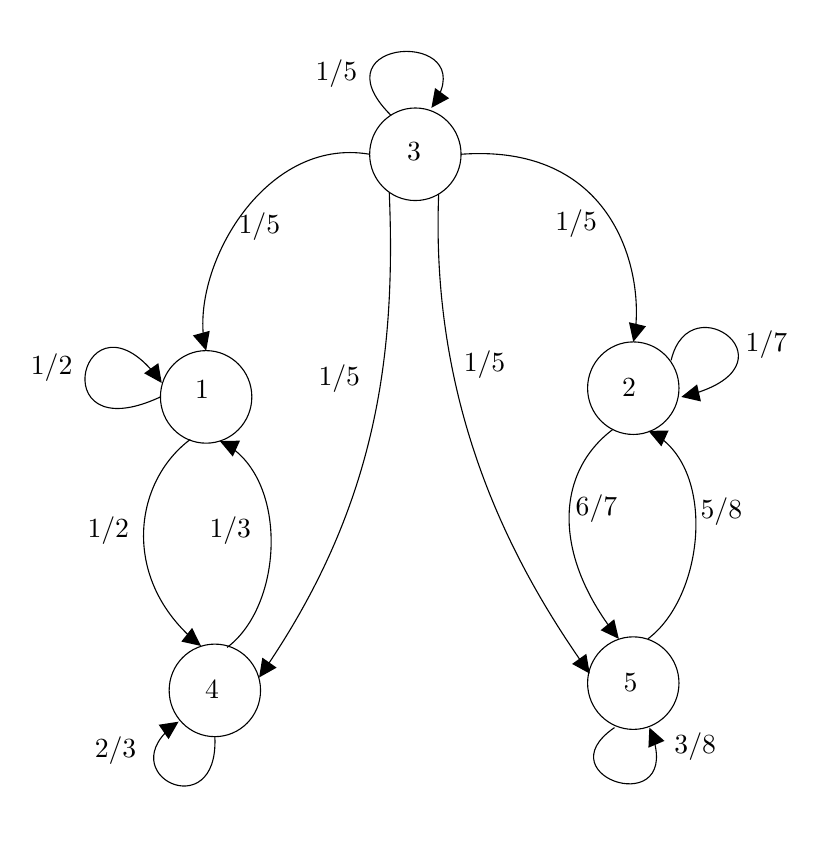
\begin{tikzpicture}[x=0.75pt,y=0.75pt,yscale=-0.7,xscale=0.7]
%uncomment if require: \path (0,714); %set diagram left start at 0, and has height of 714
%Shape: Ellipse [id:dp29836895541013164] 
\draw   (286,156.85) .. controls (286,139.26) and (300.08,125) .. (317.45,125) .. controls (334.82,125) and (348.9,139.26) .. (348.9,156.85) .. controls (348.9,174.44) and (334.82,188.7) .. (317.45,188.7) .. controls (300.08,188.7) and (286,174.44) .. (286,156.85) -- cycle ;
%Shape: Ellipse [id:dp4858180433459096] 
\draw   (142,323.85) .. controls (142,306.26) and (156.08,292) .. (173.45,292) .. controls (190.82,292) and (204.9,306.26) .. (204.9,323.85) .. controls (204.9,341.44) and (190.82,355.7) .. (173.45,355.7) .. controls (156.08,355.7) and (142,341.44) .. (142,323.85) -- cycle ;
%Shape: Ellipse [id:dp10893001214881792] 
\draw   (436,317.85) .. controls (436,300.26) and (450.08,286) .. (467.45,286) .. controls (484.82,286) and (498.9,300.26) .. (498.9,317.85) .. controls (498.9,335.44) and (484.82,349.7) .. (467.45,349.7) .. controls (450.08,349.7) and (436,335.44) .. (436,317.85) -- cycle ;
%Shape: Ellipse [id:dp31584444241771226] 
\draw   (148,525.85) .. controls (148,508.26) and (162.08,494) .. (179.45,494) .. controls (196.82,494) and (210.9,508.26) .. (210.9,525.85) .. controls (210.9,543.44) and (196.82,557.7) .. (179.45,557.7) .. controls (162.08,557.7) and (148,543.44) .. (148,525.85) -- cycle ;
%Shape: Ellipse [id:dp6845584977543557] 
\draw   (436,520.85) .. controls (436,503.26) and (450.08,489) .. (467.45,489) .. controls (484.82,489) and (498.9,503.26) .. (498.9,520.85) .. controls (498.9,538.44) and (484.82,552.7) .. (467.45,552.7) .. controls (450.08,552.7) and (436,538.44) .. (436,520.85) -- cycle ;
%Curve Lines [id:da40673715992947246] 
\draw    (212.24,513.63) .. controls (288.82,402.26) and (304.45,300.14) .. (299.5,183.32) ;
\draw [shift={(209.9,517)}, rotate = 304.9] [fill={rgb, 255:red, 0; green, 0; blue, 0 }  ][line width=0.08]  [draw opacity=0] (12.5,-6.01) -- (0,0) -- (12.5,6.01) -- cycle    ;
%Curve Lines [id:da5133467038577342] 
\draw    (172.69,288.89) .. controls (161.52,237.16) and (212.5,144.11) .. (286,156.85) ;
\draw [shift={(173.45,292)}, rotate = 254.65] [fill={rgb, 255:red, 0; green, 0; blue, 0 }  ][line width=0.08]  [draw opacity=0] (12.5,-6.01) -- (0,0) -- (12.5,6.01) -- cycle    ;
%Curve Lines [id:da008345831811055193] 
\draw    (167.44,493.28) .. controls (114.6,449.49) and (123.1,382.7) .. (162.5,353.15) ;
\draw [shift={(169.9,495.27)}, rotate = 218.21] [fill={rgb, 255:red, 0; green, 0; blue, 0 }  ][line width=0.08]  [draw opacity=0] (12.5,-6.01) -- (0,0) -- (12.5,6.01) -- cycle    ;
%Curve Lines [id:da5634268603548509] 
\draw    (435.25,511.14) .. controls (385.72,441.07) and (327.59,334.04) .. (333.5,184.32) ;
\draw [shift={(437.5,514.32)}, rotate = 234.46] [fill={rgb, 255:red, 0; green, 0; blue, 0 }  ][line width=0.08]  [draw opacity=0] (12.5,-6.01) -- (0,0) -- (12.5,6.01) -- cycle    ;
%Curve Lines [id:da4259073730032066] 
\draw    (187.9,496.27) .. controls (227.3,466.72) and (230.27,378.53) .. (185,355.28) ;
\draw [shift={(182.9,354.27)}, rotate = 384.44] [fill={rgb, 255:red, 0; green, 0; blue, 0 }  ][line width=0.08]  [draw opacity=0] (12.5,-6.01) -- (0,0) -- (12.5,6.01) -- cycle    ;
%Curve Lines [id:da6577514807411684] 
\draw    (468.08,283.01) .. controls (475.64,242.78) and (457.71,148.87) .. (348.9,156.85) ;
\draw [shift={(467.45,286)}, rotate = 283.29] [fill={rgb, 255:red, 0; green, 0; blue, 0 }  ][line width=0.08]  [draw opacity=0] (12.5,-6.01) -- (0,0) -- (12.5,6.01) -- cycle    ;
%Curve Lines [id:da329541870026538] 
\draw    (142,323.85) .. controls (58.35,362.99) and (88.88,241.85) .. (141.3,312.08) ;
\draw [shift={(142.9,314.27)}, rotate = 234.51] [fill={rgb, 255:red, 0; green, 0; blue, 0 }  ][line width=0.08]  [draw opacity=0] (12.5,-6.01) -- (0,0) -- (12.5,6.01) -- cycle    ;
%Curve Lines [id:da3393212160499588] 
\draw    (493.5,298.66) .. controls (506.37,243.94) and (584.91,303.18) .. (503.03,323.29) ;
\draw [shift={(500.5,323.88)}, rotate = 347.23] [fill={rgb, 255:red, 0; green, 0; blue, 0 }  ][line width=0.08]  [draw opacity=0] (12.5,-6.01) -- (0,0) -- (12.5,6.01) -- cycle    ;
%Curve Lines [id:da7968400462935867] 
\draw    (477.5,490.39) .. controls (516.9,460.84) and (525.1,371.56) .. (480,348.28) ;
\draw [shift={(477.9,347.27)}, rotate = 384.44] [fill={rgb, 255:red, 0; green, 0; blue, 0 }  ][line width=0.08]  [draw opacity=0] (12.5,-6.01) -- (0,0) -- (12.5,6.01) -- cycle    ;
%Curve Lines [id:da49532662514959913] 
\draw    (455.47,487.82) .. controls (411.57,431.68) and (414.1,375.7) .. (453.5,346.15) ;
\draw [shift={(457.5,490.39)}, rotate = 231.1] [fill={rgb, 255:red, 0; green, 0; blue, 0 }  ][line width=0.08]  [draw opacity=0] (12.5,-6.01) -- (0,0) -- (12.5,6.01) -- cycle    ;
%Curve Lines [id:da618838807270425] 
\draw    (179.45,557.7) .. controls (182.46,620.43) and (105.86,583.53) .. (152.3,548.96) ;
\draw [shift={(154.5,547.39)}, rotate = 505.54] [fill={rgb, 255:red, 0; green, 0; blue, 0 }  ][line width=0.08]  [draw opacity=0] (12.5,-6.01) -- (0,0) -- (12.5,6.01) -- cycle    ;
%Curve Lines [id:da7726575310463464] 
\draw    (479.68,554.36) .. controls (503.45,616.53) and (404.27,585.93) .. (454.51,551.46) ;
\draw [shift={(478.51,551.46)}, rotate = 67.01] [fill={rgb, 255:red, 0; green, 0; blue, 0 }  ][line width=0.08]  [draw opacity=0] (12.5,-6.01) -- (0,0) -- (12.5,6.01) -- cycle    ;
%Curve Lines [id:da7210031613710599] 
\draw    (330.71,121.65) .. controls (363.66,70.1) and (246.61,75.98) .. (300.51,129.88) ;
\draw [shift={(328.51,124.88)}, rotate = 306.03] [fill={rgb, 255:red, 0; green, 0; blue, 0 }  ][line width=0.08]  [draw opacity=0] (12.5,-6.01) -- (0,0) -- (12.5,6.01) -- cycle    ;
% Text Node
\draw (164,311.21) node [anchor=north west][inner sep=0.75pt]   [align=left] {{\normalsize 1}};
% Text Node
\draw (458,309.21) node [anchor=north west][inner sep=0.75pt]   [align=left] {{\normalsize 2}};
% Text Node
\draw (171,517.21) node [anchor=north west][inner sep=0.75pt]   [align=left] {{\normalsize 4}};
% Text Node
\draw (459,512.21) node [anchor=north west][inner sep=0.75pt]   [align=left] {{\normalsize 5}};
% Text Node
\draw (310,147.21) node [anchor=north west][inner sep=0.75pt]   [align=left] {{\normalsize 3}};
% Text Node
\draw (51,292.21) node [anchor=north west][inner sep=0.75pt]   [align=left] {{\normalsize 1/2}};
% Text Node
\draw (90,404.21) node [anchor=north west][inner sep=0.75pt]   [align=left] {{\normalsize 1/2}};
% Text Node
\draw (543,276.21) node [anchor=north west][inner sep=0.75pt]   [align=left] {{\normalsize 1/7}};
% Text Node
\draw (174,404.21) node [anchor=north west][inner sep=0.75pt]   [align=left] {{\normalsize 1/3}};
% Text Node
\draw (194,195.21) node [anchor=north west][inner sep=0.75pt]   [align=left] {{\normalsize 1/5}};
% Text Node
\draw (426,389.21) node [anchor=north west][inner sep=0.75pt]   [align=left] {{\normalsize 6/7}};
% Text Node
\draw (512,391.21) node [anchor=north west][inner sep=0.75pt]   [align=left] {{\normalsize 5/8}};
% Text Node
\draw (95,556.21) node [anchor=north west][inner sep=0.75pt]   [align=left] {{\normalsize 2/3}};
% Text Node
\draw (494,553.21) node [anchor=north west][inner sep=0.75pt]   [align=left] {{\normalsize 3/8}};
% Text Node
\draw (247,90.21) node [anchor=north west][inner sep=0.75pt]   [align=left] {{\normalsize 1/5}};
% Text Node
\draw (249,300.21) node [anchor=north west][inner sep=0.75pt]   [align=left] {{\normalsize 1/5}};
% Text Node
\draw (349,290.21) node [anchor=north west][inner sep=0.75pt]   [align=left] {{\normalsize 1/5}};
% Text Node
\draw (412,193.21) node [anchor=north west][inner sep=0.75pt]   [align=left] {{\normalsize 1/5}};
\end{tikzpicture}

		
		
		\\  
		&\\
		&\\
		\hline
		\multirow{3}{*}{Checking whether the  } & \\
		& Here,\\states 3 and 1 are in the
		& State 1 is accessible from the state 3.\\same communicating class
	    	& But, State 3 is not accessible from the state 1\\
	    	& \qquad \qquad \qquad i.e.  $3 \rightarrow 1$,  $1 \nrightarrow 3$\\
	    	& \qquad \qquad \qquad$\implies \boxed{3 \nleftrightarrow 1}$\\
	    	&\\ 
	    	&Therefore, 3 and 1 are not in the same communicating class.\\
	   	&\\
	   	\hline
	   \multirow{3}{*}{Checking whether the  } & \\
		& Here,\\states 1 and 4 are in the
		& State 1 is accessible from the state 4.\\same communicating class
	    	& Also, State 4 is accessible from the state 1\\
	    	& \qquad \qquad \qquad i.e.  $3 \rightarrow 1$,  $1 \rightarrow 3$\\
	   	& \qquad \qquad \qquad$\implies \boxed{3 \leftrightarrow 1}$\\
	    	&\\ 
	    	&Therefore, 1 and 4 are in the same communicating class.\\	   	
	   	&\\	   	
	   	\hline
	   	\multirow{3}{*}{Checking whether the  } & \\
		& Here,\\states 4 and 2 are in the
		& State 2 is not accessible from the state 4.\\same communicating class
	    	& Also, State 4 is not accessible from the state 2\\
	    	& \qquad \qquad \qquad i.e.  $4 \nrightarrow 2$,  $2 \nrightarrow 4$\\
	    	\hline
	    	&\\	    	
	   	& \qquad \qquad \qquad$\implies \boxed{4 \nleftrightarrow 2}$\\
	    	&Therefore, 4 and 2 are not in the same communicating class.\\
	   	&\\
	   	\hline
	   	\multirow{3}{*}{Checking whether the  } & \\
		& Here,\\states 2 and 5 are in the
		& State 2 is accessible from the state 5.\\same communicating class
	    	& Also, State 5 is accessible from the state 2\\
	    	& \qquad \qquad \qquad i.e.  $5 \rightarrow 2$,  $2 \rightarrow 5$\\
	   	& \qquad \qquad \qquad$\implies \boxed{2 \leftrightarrow 5}$\\
	    	&\\
	    	&Therefore, 2 and 5 are in the same communicating class.\\
	   	&\\
	   	\hline
	   	\multirow{3}{*}{Conclusion} & \\
	   	&Communication classes are:\\
	   	&\\
	   	& \qquad \qquad \qquad$\boxed{S=\{1,4\}\cup \{3\} \cup \{2,5\}}$\\
	   	&\\
		&Option 2) and 4) are true.\\
	   	&\\
	   	\hline
\caption{Solution}
\label{eq:solutions/2017/dec/105/table1}
    \end{longtable}
%\end{table*}
\twocolumn


%\twocolumn 
%
\item $A$ and $B$ play a game of tossing a fair coin. $A$ starts the game by tossing the coin once and $B$ then tosses the coin twice, followed by $A$ tossing the coin once and $B$ tossing the coin twice and this continues until a head turns up. Whoever gets the first head wins the game. Then, 
\begin{enumerate}
    \item $P(B$ Wins) $> P(A$ Wins)
    \item $P(B$ Wins) $= 2P(A$ Wins)
    \item $P(A$ Wins) $> P(B$ Wins)
    \item $P(A$ Wins) $= 1-P(B$ Wins)
\end{enumerate}
%
%
\solution
Given, a fair coin is tossed till heads turns up.
\begin{align}
\tag{104.1}
\label{dec2016-104eq:0}
    p=\dfrac{1}{2},q=\dfrac{1}{2}
\end{align}
Let's define a Markov chain $\{X_{n},n=0,1,2,\dots\}$, where $X_{n}\in S=\{1,2,3,4,5\}$, such that
\begin{table}[h!]
\centering
\caption{States and their notations}
\label{dec2016-104table:1}
\begin{tabular}{|c|c|}
    \hline
    Notation & State \\
    \hline
    $S=1$ & $A$'s turn\\[1ex]
    \hline
    $S=2$ & $B$'s first turn\\[1ex]
    \hline
    $S=3$ & $B$'s second turn\\[1ex]
    \hline
    $S=4$ & $A$ wins\\[1ex]
    \hline
    $S=4$ & $B$ wins\\[1ex]
    \hline
\end{tabular}
\end{table}
The state transition matrix for the Markov chain is
\begin{align}
\tag{104.2}
\label{dec2016-104eq:p}
    P=\begin{blockarray}{cccccc}
&1 & 2 & 3 & 4 & 5 \\
\begin{block}{c[ccccc]}
  1 & 0 & 0.5 & 0 & 0.5 & 0 \\
  2 & 0 & 0 & 0.5 & 0 & 0.5 \\
  3 & 0.5 & 0 & 0 & 0 & 0.5 \\
  4 & 0 & 0 & 0 & 1 & 0 \\
  5 & 0 & 0 & 0 & 0 & 1 \\
\end{block}
\end{blockarray}
\end{align}
Clearly, the states $1,2,3$ are transient, while $4,5$ are absorbing. The standard form of a state transition matrix is
\begin{align}
\tag{104.3}
\label{dec2016-104eq:std}
    P=\begin{blockarray}{ccc}
&A & N \\
\begin{block}{c[cc]}
  A & I & O  \\
  N & R & Q \\
\end{block}
\end{blockarray}
\end{align}
where,
\begin{table}[h!]
\centering
\caption{Notations and their meanings}
\label{dec2016-104table:2}
\begin{tabular}{|c|c|}
    \hline
    Notation & Meaning \\
    \hline
    $A$ & All absorbing states\\[1ex]
    \hline
    $N$ & All non-absorbing states\\[1ex]
    \hline
    $I$ & Identity matrix\\[1ex]
    \hline
    $O$ & Zero matrix\\[1ex]
    \hline
    $R,Q$ & Other submatices\\[1ex]
    \hline
\end{tabular}
\end{table}
Converting \eqref{dec2016-104eq:p} to standard form, we get
\begin{align}
\tag{104.4}
\label{dec2016-104eq:pstd}
    P=\begin{blockarray}{cccccc}
&4 & 5 & 1 & 2 & 3 \\
\begin{block}{c[ccccc]}
  4 & 1 & 0 & 0 & 0 & 0 \\
  5 & 0 & 1 & 0 & 0 & 0 \\
  1 & 0.5 & 0 & 0 & 0.5 & 0 \\
  2 & 0 & 0.5 & 0 & 0 & 0.5 \\
  3 & 0 & 0.5 & 0.5 & 0 & 0 \\
\end{block}
\end{blockarray}
\end{align}
From \eqref{dec2016-104eq:pstd},
\begin{align}
\tag{104.5}
\label{dec2016-104eq:r,q}
    R=\begin{bmatrix}
    0.5 & 0\\
    0 & 0.5\\
    0 & 0.5\\
    \end{bmatrix},
    Q=\begin{bmatrix}
    0 & 0.5 & 0\\
    0 & 0 & 0.5\\
    0.5 & 0 & 0\\
    \end{bmatrix}
\end{align}
\newpage
The limiting matrix for absorbing Markov chain is
\begin{align}
\tag{104.6}
\label{dec2016-104eq:pbar}
    \bar P=\begin{bmatrix}
    I & O\\
    FR & O\\
    \end{bmatrix}
\end{align}
where,
\begin{align}
\tag{104.7}
\label{dec2016-104eq:f}
    F=(I-Q)^{-1}
\end{align}
is called the fundamental matrix of $P$. \\
On solving, we get
\begin{align}
\tag{104.8}
\label{dec2016-104eq:ans}
    \bar P=\begin{blockarray}{cccccc}
&4 & 5 & 1 & 2 & 3 \\
\begin{block}{c[ccccc]}
    4 & 1 & 0 & 0 & 0 & 0 \\
    5 & 0 & 1 & 0 & 0 & 0 \\
    1 & 0.5714 & 0.4285 & 0 & 0 & 0 \\
    2 & 0.1428 & 0.8571 & 0 & 0 & 0 \\
    3 & 0.2857 & 0.7142 & 0 & 0 & 0 \\
   \end{block}
\end{blockarray}
\end{align}
A element $\bar p_{ij}$ of $\bar P$ denotes the absorption probability in state $j$, starting from state $i$. Then,
\begin{enumerate}
    \item $Pr(A$ wins)=$\bar p_{14}\approx0.5714$
    \item $Pr(B$ wins)=$\bar p_{15}\approx0.4285$
\end{enumerate}
\begin{align}
\tag{104.9}
\therefore \bar p_{14} > \bar p_{15}
\end{align}
Also, in $\bar P$, all the terms in every row should sum to 1.
\begin{align}
\tag{104.10}
\Rightarrow \bar p_{14} + \bar p_{15}+ 0+0+0=1\\
\tag{104.11}
\therefore \bar p_{14}=1-\bar p_{15}
\end{align}
Therefore, options $3),4)$ are correct.\\
\begin{figure}[h]
\caption*{\textbf{Markov chain diagram}}
\centering
\begin{tikzpicture}
    % Setup the style for the states
        \tikzset{node style/.style={state, 
                                    minimum width=1.5cm,
                                    line width=1mm,
                                    fill=gray!20!white}}
        % Draw the states
        \node[node style] at (3, -4)      (bull)     {1};
        \node[node style] at (0, -8)      (bear)     {2};
        \node[node style] at (6, -8) (stagnant) {3};
        \node[node style] at (3, 0) (over1) {4};
        \node[node style] at (3, -12) (over2) {5};
        % Connect the states with arrows
        \draw[every loop,
              auto=right,
              line width=0.7mm,
              >=latex,
              draw=orange,
              fill=orange]
            (stagnant)     edge[bend right=20]            node {$\dfrac{1}{2}$} (bull)
            (stagnant)     edge[bend left=20]            node {$\dfrac{1}{2}$} (over2)
            (bull)     edge[bend right=20] node {$\dfrac{1}{2}$} (bear)
            (bull)     edge node {$\dfrac{1}{2}$} (over1)
            (bear)     edge[bend right=20] node {$\dfrac{1}{2}$} (over2)
            (bear)     edge node {$\dfrac{1}{2}$} (stagnant)
            (over1) edge[loop above]             node  {1} (over1)
            (over2) edge[loop below]             node  {1} (over2);
\end{tikzpicture}
\end{figure}
\item Consider a Markov chain with state space {1,2,....,100}. Suppose states 2i and 2j communicate with each other and states 2i-1 and 2j-1 communicate with each other for every i,j = 1,2,...,50. Further suppose that $p^{(2)}_{3,3}$ > 0,$p^{(3)}_{4,4}$ > 0 and $p^{(7)}_{2,5}$ > 0. Then 
\begin{enumerate}
\item The Markov chain is irreducible.
\item The Markov chain is aperiodic.
\item State 8 is recurrent.
\item State 9 is recurrent.
\end{enumerate}
\solution
\input{solutions/2014/dec/106/LaTex/Assignment_7.tex}


\end{enumerate}
